%%
%% kit-prog-tutorial
%%
%% Slides for my Java programming tutorial at KIT using LaTeX beamer.
%%
%% Copyright (c) 2015-2016 YouniS Bensalah <younis.bensalah@gmail.com>
%%
%% This work is released to the public domain.
%% For the full copyright and license information, please view the LICENSE file.
%%

\documentclass[18pt]{beamer}

\usepackage{templates/beamerthemekit}

\usepackage[utf8]{inputenc}
\usepackage{hyperref}
\usepackage{listings}
\usepackage{xcolor}
\usepackage{colortbl}
\usepackage{array}
\usepackage{amsmath}
\usepackage{amssymb}
\usepackage{mathrsfs}
\usepackage{eurosym}

\titleimage{road}

\definecolor{lime}{HTML}{8FFF53}

\newcommand{\tagline}{Recursion \& Java API}

\newcommand{\quotes}[1]{``#1''}

\title[Programmieren\hspace{2.5pt}--\hspace{2.5pt}\tagline]{\tagline}
\subtitle{Programmieren~\textbar~Tutorium 32}

\author{YouniS Bensalah}
\date{23. Januar 2017}

\institute{Chair for Software Design and Quality}

\usepackage[citestyle=authoryear,bibstyle=numeric,hyperref,backend=biber]{biblatex}
\addbibresource{templates/example.bib}
\bibhang1em

\begin{document}

% remove annoying figure prefix in caption
\setbeamertemplate{caption}{\raggedright\insertcaption\par}

\selectlanguage{english}

\begin{frame}
    \titlepage
\end{frame}

% \begin{frame}{Heute}
%     \tableofcontents
% \end{frame}

\begin{frame}{Divide and Conquer}
    \begin{itemize}
        \item \quotes{Teile und herrsche}
        \item Wichtiger Ansatz in der Algorithmik
        \vspace{.2in}
        \begin{enumerate}
            \item Teile Problem so lange in kleinere Teilprobleme, bis diese einfach lösbar sind
            \item Löse die einzelnen Teilprobleme
            \item Füge Teillösungen zu Lösung des Gesamtproblems zusammen
        \end{enumerate}
    \end{itemize}
\end{frame}

\begin{frame}{Rekursion}
    \begin{itemize}
        \item \textbf{Prinzip der Rekursion}
        \begin{itemize}
            \item Funktion kann sich selbst aufrufen
            \item Führe gleiches Berechnungsmuster immer wieder mit kleineren Eingabedaten aus, bis Problem trivial ist
        \end{itemize}
        \pause
        \vspace{.2in}
        \item Rekursion ist Form von \textit{Divide and Conquer}
    \end{itemize}
\end{frame}

\begin{frame}{Rekursion}
    Siehe \quotes{Rekursion}.
\end{frame}

\begin{frame}{Rekursion: Fakultät}
    \begin{exampleblock}{}
        \begin{itemize}
            \item Berechnung der Fakultät einer (nicht negativen, ganzen) Zahl:\\
            \vspace{.2in}
            $
            n! = \prod\limits_{i=1}^{n} =
                \begin{cases}
                    n \cdot (n-1)! & \text{if\qquad} n > 0 \\
                    1 & \text{if\qquad} n = 0
                \end{cases}
            $
        \end{itemize}
    \end{exampleblock}
\end{frame}

\begin{frame}[fragile]{Rekursion: Fakultät}
    \begin{exampleblock}{}
        \begin{lstlisting}[language=Java,basicstyle=\scriptsize]
int factorial(int n) {
    if (n > 0) {
        return n * factorial(n - 1);
    } else {
        return 1;
    }
}
        \end{lstlisting}

    \end{exampleblock}

\end{frame}

\begin{frame}[fragile]{Rekursion: Ackermannfunktion}
    \begin{exampleblock}{}
        $
        \mathscr{A}(m, n) :=
        \begin{cases}
            n+1 & \text{if\quad} m = 0\\
            \mathscr{A}(m-1, 1) & \text{if\quad} m > 0 \text{\,and\,} n = 0\\
            \mathscr{A}(m-1, \mathscr{A}(m, n-1)) & \text{if\quad} m > 0 \text{\,and\,} n > 0
        \end{cases}
        $
    \end{exampleblock}
    \pause
    \begin{itemize}
        \item $\mathscr{A}(1, 1) = 3$
        \item $\mathscr{A}(1, 2) = 4$
        \item $\mathscr{A}(2, 3) = 9$
        \item $\mathscr{A}(2, 4) = 11$
    \end{itemize}
\end{frame}

\begin{frame}{Rekursion: Ackermannfunktion}
    \begin{itemize}
        \item $\mathscr{A}(4, 2)$ ist eine Zahl mit \textbf{19729} Dezimalstellen
    \end{itemize}
\end{frame}


\subsubsection{Iteration vs. Rekursion}

\begin{frame}[fragile]{Iteration vs. Rekursion}
    Alternativ zur rekursiven Variante von \texttt{factorial()}\dots
    \begin{exampleblock}{}
        \begin{lstlisting}[language=Java,basicstyle=\scriptsize]
int factorial(int n) {
    int result = 1;
    for (int i = 2; i <= n; ++i) {
        result *= i;
    }
    return result;
}
        \end{lstlisting}

    \end{exampleblock}
\end{frame}

\begin{frame}{Zusammenfassung}
    \begin{itemize}
        \item \textbf{Rekursion} kann speicheraufwendig werden, da jedes Mal eine neue Instanz der Methode aufgerufen wird
        \begin{itemize}
            \item Stack kann überlaufen!
        \end{itemize}
        \item Nicht immer klar, ob die Berechnung terminiert
        \item Rekursion ist bei manchen Problemen eine elegante Lösung
        \item Es gibt nicht immer eine \quotes{iterative Lösung} (siehe \textit{Ackermannfunktion})
    \end{itemize}
\end{frame}

\begin{frame}{Java API}
    \begin{itemize}
        \item Die \textbf{Java API} ist eine Sammlung von Klassen/Paketen für häufig benötigte Funktionalitäten

        \begin{itemize}
            \item \texttt{java.lang}: Basisfunktionalität
            \item \texttt{java.util}: Java Collections Framework
            \item \texttt{java.io}: Ein- und Ausgabe
        \end{itemize}

        \vspace{.2in}

        \item Das \textbf{Java Collections Framework} enthält u.a.
        \begin{itemize}
            \item \texttt{Map<K,V>}, \texttt{Set<E>}\dots
            \item \texttt{Queue<E>}, \texttt{Deque<E>}, \texttt{Stack<E>}\dots
            \item \texttt{List<E>}, \texttt{LinkedList<E>}\dots
        \end{itemize}

        \vspace{.2in}

        \item \quotes{Das Rad muss nicht neu erfunden werden.}

    \end{itemize}
\end{frame}

\begin{frame}{Sets und Maps}
    \begin{block}{}
        \begin{itemize}
            \item Ein \textbf{Set} stellt eine Menge (im mathematischen Sinne) dar
            \item Sammlung von Objekten, \textit{ohne Duplikate}
        \end{itemize}
    \end{block}

    \begin{block}{}
        \begin{itemize}
            \item Eine \textbf{Map} stellt eine Abbildung von Schlüsseln (keys) auf Werte (values) dar
            \item Beispiel: \texttt{String} als key, \texttt{Student} als value
        \end{itemize}

    \end{block}
\end{frame}

\begin{frame}[fragile]{Sets}
    \begin{lstlisting}[language=Java]
Set<String> names = new HashSet<>();

names.add("Alice");
names.add("Eve");
names.add("Bob");
names.add("Eve");

it = names.iterator();
String name;
while (it.hasNext()) {
    name = it.next();
    System.out.println(name);
}
    \end{lstlisting}

\end{frame}

\begin{frame}[fragile]{Sets}
    \begin{exampleblock}{}
        \begin{lstlisting}[language=Java]
Bob
Eve
Alice
        \end{lstlisting}
    \end{exampleblock}

\end{frame}


\begin{frame}[fragile]{Maps}
    \begin{lstlisting}[language=Java]
Map<String, Integer> mountains = new HashMap<>();

mountains.put("Everest", 8848);
mountains.put("K2", 8611);
mountains.put("Kangchenjunga", 8586);
mountains.put("Lhotse", 8516);

System.out.println(mountains.get("Everest"));
    \end{lstlisting}
\end{frame}

\begin{frame}[fragile]{Maps}

    \begin{exampleblock}{}
        \begin{lstlisting}[language=Java]
8848
        \end{lstlisting}

    \end{exampleblock}
\end{frame}


\begin{frame}[fragile]{Stack}
    \begin{lstlisting}[language=Java]
Stack<String> books = new Stack<>();

books.push("Modern Operating Systems");
books.push("The Magic Garden Explained");

System.out.println(books.peek());
books.pop();

books.push("The Art of Game Design");

String next;
while (!books.empty()) {
    next = books.pop();
    System.out.println(next);
}
    \end{lstlisting}

\end{frame}

\begin{frame}[fragile]{Stack}
    \begin{exampleblock}{}
        \begin{lstlisting}[language=Java]
The Magic Garden Explained
The Art of Game Design
Modern Operating Systems
        \end{lstlisting}
    \end{exampleblock}

\end{frame}

\begin{frame}{Read the fine manual}
    \Large{\url{https://docs.oracle.com/javase/8/docs/api}}
\end{frame}

\appendix
\beginbackup

\begin{frame}{Fragen?}
    \begin{figure}
        
\includegraphics[scale=.6]{img/additionalquestions.jpg}
    \end{figure}
\end{frame}

\begin{frame}{Bis nächste Woche!}
    \begin{figure}
        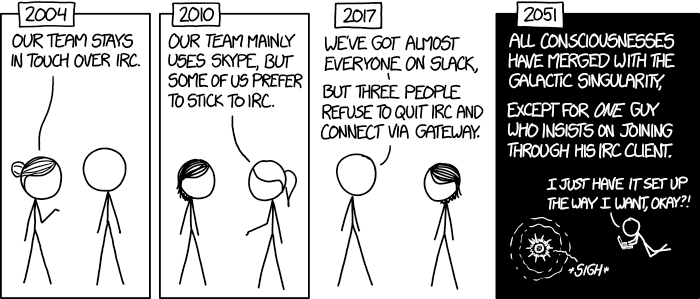
\includegraphics[scale=.4]{img/team_chat.png}
        \caption{\footnotesize{xkcd.com}}
    \end{figure}
\end{frame}

\backupend

\end{document}
